%
%  image_data.tex
%
% 
%
\documentclass[xcolor=dvipsnames, 9pt]{beamer}

\usepackage{amssymb}
\usepackage{amsfonts}
\usepackage{amsmath}
\usepackage{hyperref}
\usepackage{natbib}
\usepackage{color}
\usepackage{pdfsync}
\usepackage{chancery}
\usepackage{movie15}
\usepackage{pgfpages}
\usepackage{fancyvrb}
\usepackage{colortbl}
\usepackage{multirow}

\usepackage{graphicx}
\graphicspath{{../../images/figures/}{../../images/logos/}{../../images/graphs/}/}

\usepackage{beamerthemesplit}
\usetheme{Copenhagen}
\definecolor{title}{RGB}{128,148,182}
\usecolortheme[named=title]{structure} 
\setbeamertemplate{headline}{}
\setbeamertemplate{navigation symbols}{}
\setbeamertemplate{itemize items}[triangle]
\setbeamertemplate{enumerate items}[default]
\setbeamertemplate{footline}[page number]{}
%\setbeameroption{show notes on second screen}


\usepackage{listings}
%\usepackage{listings,arev}
\definecolor{keywords}{RGB}{128,148,182}
\definecolor{comments}{RGB}{60,179,113}
\lstset{numbers=left,
        showstringspaces=false,
        numberstyle=\tiny,
        %frame=leftline,
        numbersep=4.5pt,
  keywordstyle=\color{keywords}\bfseries,
  commentstyle=\color{YellowOrange}\emph
}

\newenvironment{code}{\begin{semiverbatim} \begin{footnotesize}}
{\end{footnotesize}\end{semiverbatim}}


\newcommand{\R}{\mathbb{R}}
\renewcommand{\d}{\mathsf{d}}
\newcommand{\dd}{\partial}
\newcommand{\E}{\mathsf{E}}
\newcommand{\bb}{\mathbf}

\title{Working with Image Data\\Bootcamp Section 1}
\author{Joseph Adler, Drew Conway, Jake Hofman, Hilary Mason}
\date{February 1, 2011}

\begin{document} 

\begin{frame}[plain]
  \titlepage 
  
  \tiny
  \href{http://creativecommons.org/licenses/by-sa/3.0/us/}{
\includegraphics[width=1cm]{ccbysa}}

  Creative Commons Attribution-Share Alike 3.0
\end{frame}


\AtBeginSection[]{
  \begin{frame}
    \frametitle{Outline}
    \tableofcontents[currentsection]
  \end{frame}
}

\begin{frame}
  \frametitle{Acquiring image data}

  \begin{center}
  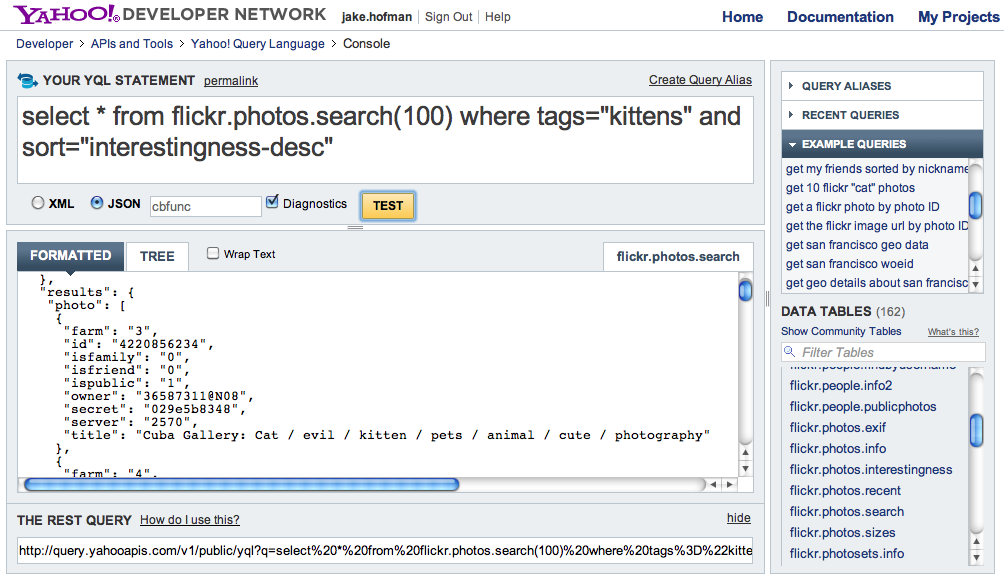
\includegraphics[width=\textwidth]{yql_console.png}
  \end{center}

\end{frame}


\begin{frame}
  \frametitle{Image features}

  \begin{center}
  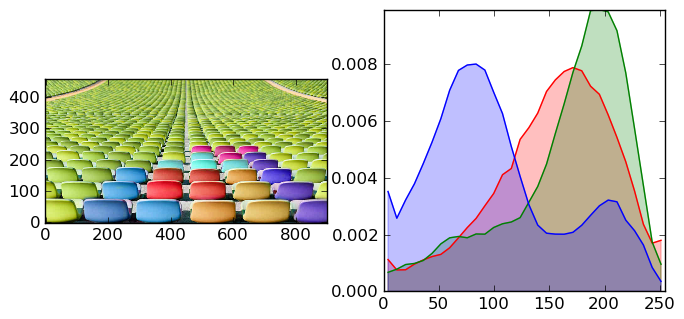
\includegraphics[width=\textwidth]{../../code/image_data/chairs_32.png}
  \end{center}

\end{frame}


\begin{frame}
  \frametitle{Clustering pixels}

  \begin{center}
    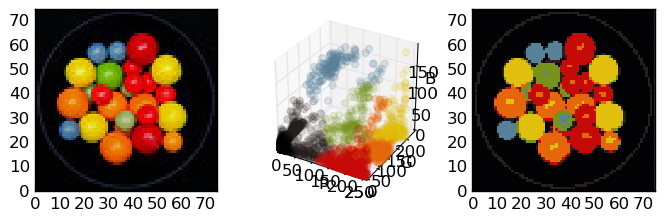
\includegraphics[width=\textwidth]{../../code/image_data/candy_clustered.png}
  \end{center}

\end{frame}


\begin{frame}
  \frametitle{Clustering images}

  \begin{center}
    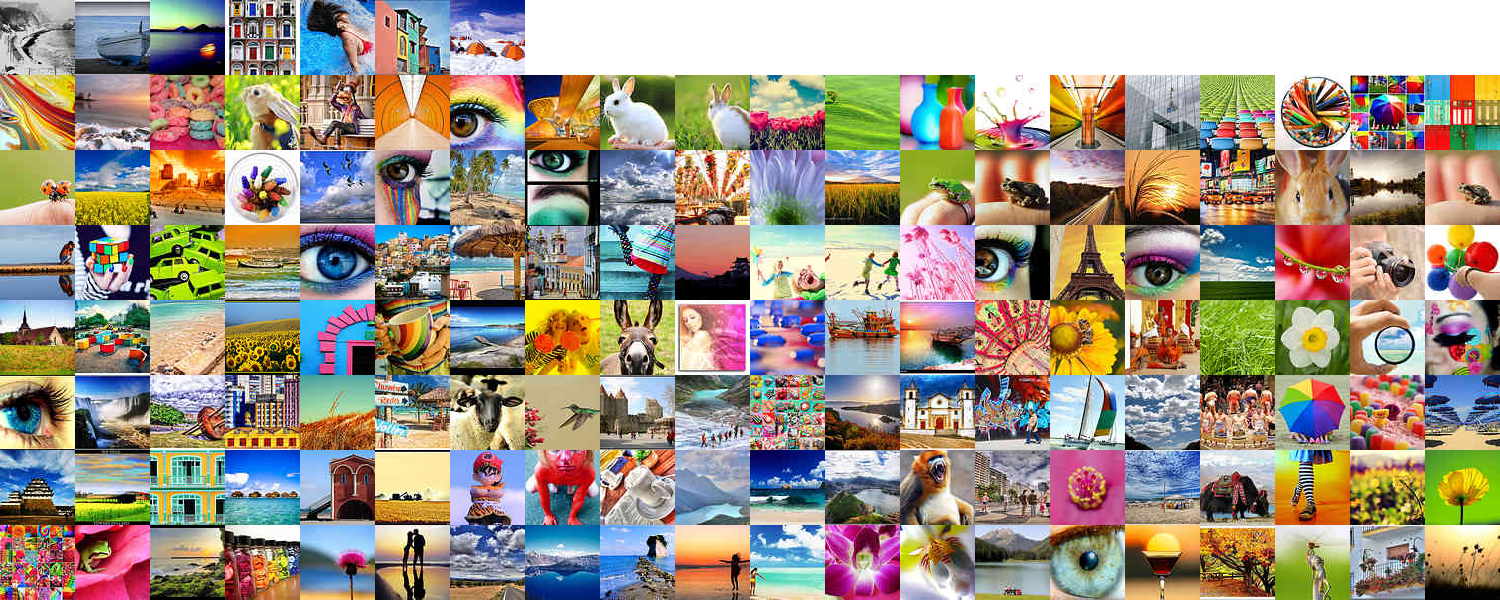
\includegraphics[width=0.65\textwidth]{../../code/image_data/flickr_vivid_cluster_1.png}
    \vskip10pt
    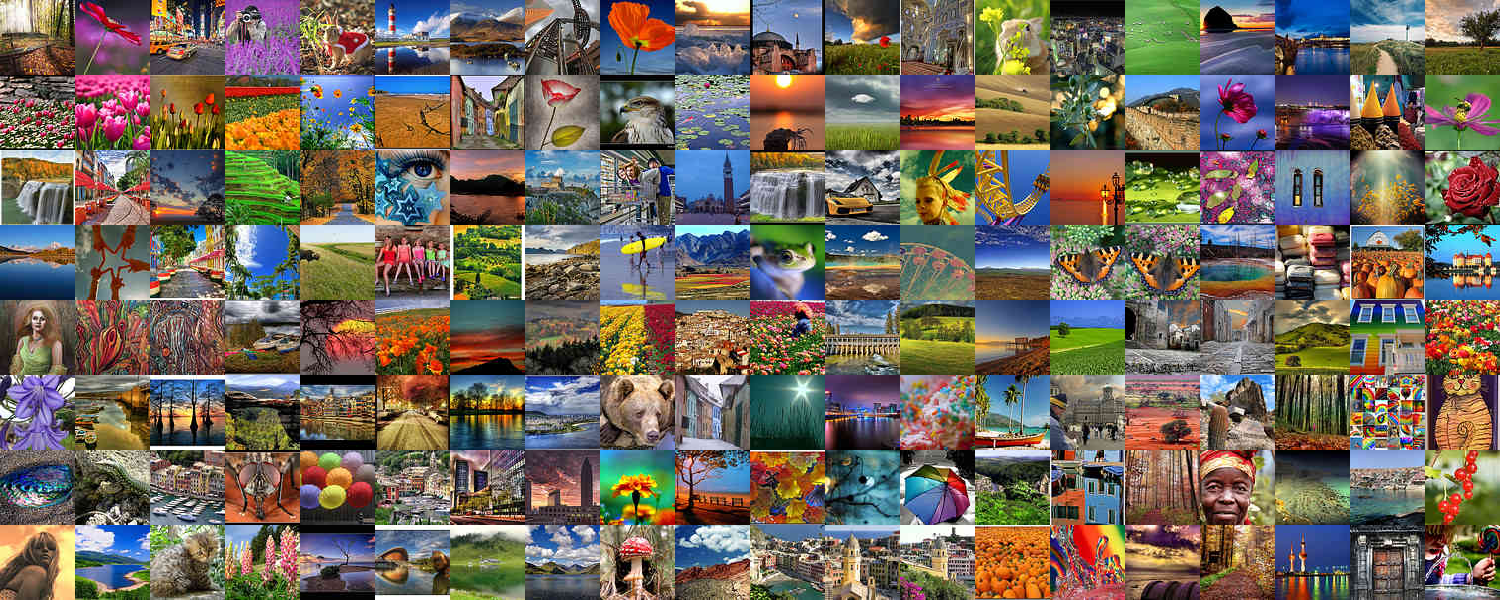
\includegraphics[width=0.65\textwidth]{../../code/image_data/flickr_vivid_cluster_2.png}
    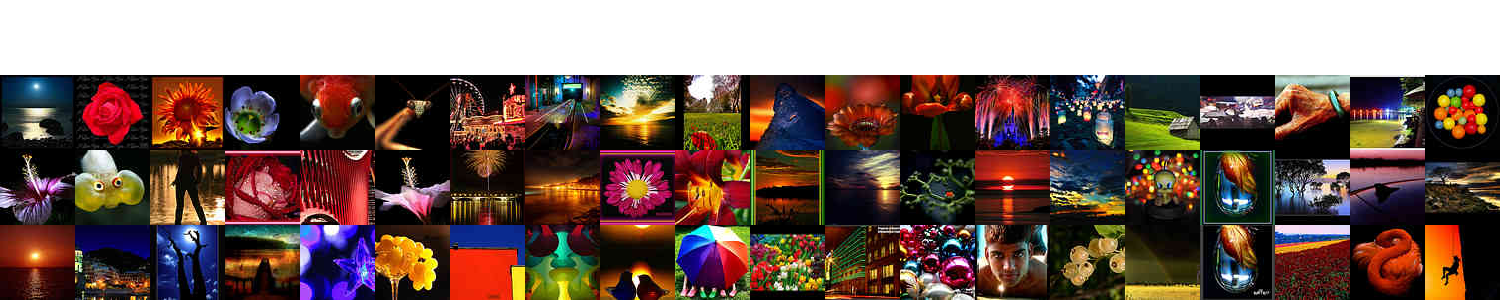
\includegraphics[width=0.65\textwidth]{../../code/image_data/flickr_vivid_cluster_3.png}

    %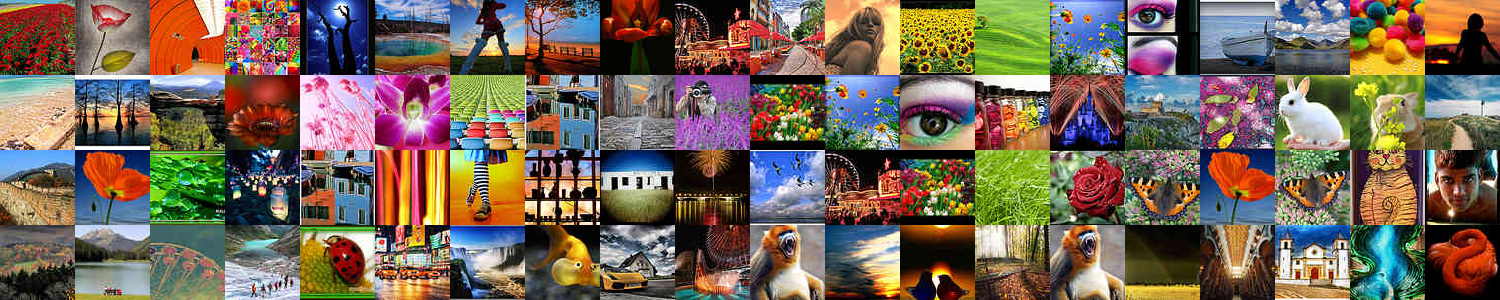
\includegraphics[width=\textwidth]{../../code/image_data/flickr_vivid_sample.png}
  \end{center}

\end{frame}


\begin{frame}
  \frametitle{Classifying images}

  \begin{center}
    
\includegraphics[width=0.5\textwidth]{ocr.png} \\
  %\only<1>{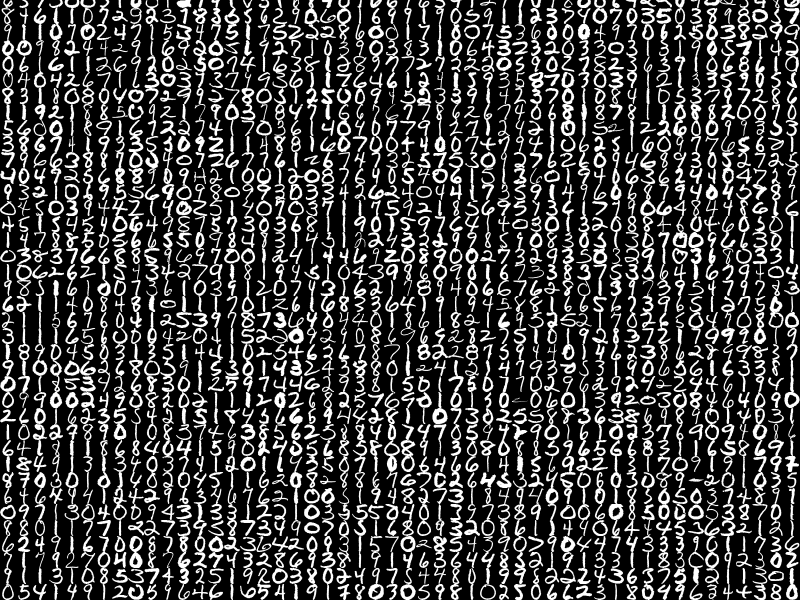
\includegraphics[width=0.75\textwidth]{../../code/image_data/sample_digits.png}}
  %\only<2>{
\includegraphics[width=32pt]{../../code/image_data/sample_digit.png} \\
  \Huge{$\downarrow$} \\
  \Huge{0 \hskip10pt 5 \hskip10pt 4 \hskip10pt 1 \hskip10pt 4 \hskip10pt 9}
  \end{center}

\end{frame}


\section{Acquiring image data}
\begin{frame}[fragile]
  \frametitle{Simple screen scraping}

    \begin{block}{One-liner to scrape images from a webpage}
        \begin{lstlisting}[language=bash]
 wget -O- http://bit.ly/gpCSQi | 
   tr ''\''"=' '\n' | 
   egrep '^http.*(png|jpg|gif)' | 
   xargs wget 
        \end{lstlisting}
    \end{block} 

    \pause
    \begin{itemize}
      \item get page source
      \item translate quotes and = to newlines
      \item match urls with image extensions
      \item download qualifying images
    \end{itemize}

\end{frame}


\begin{frame}
  \frametitle{``cat flickr \big| xargs wget''?}

  \begin{center}
    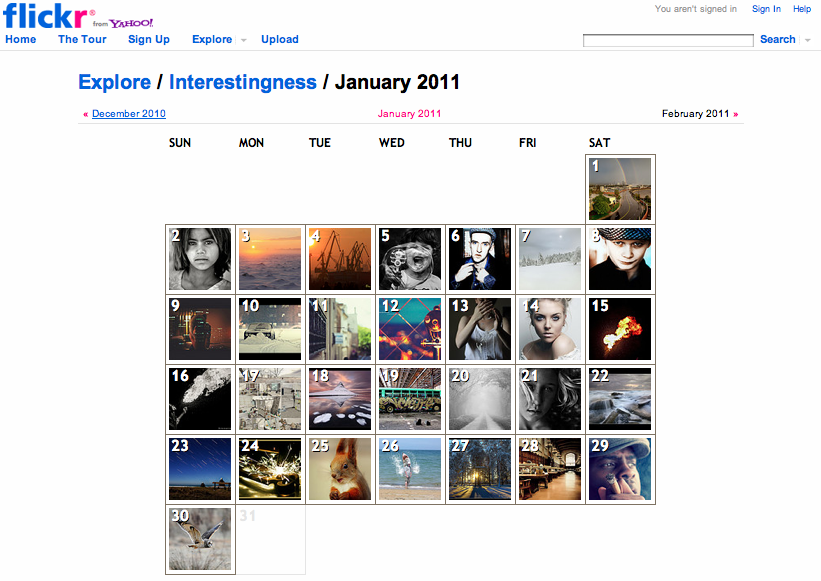
\includegraphics[width=\textwidth]{flickr_201101.png}
  \end{center}

\end{frame}


\begin{frame}
  \frametitle{Flickr API}

  \begin{center}
    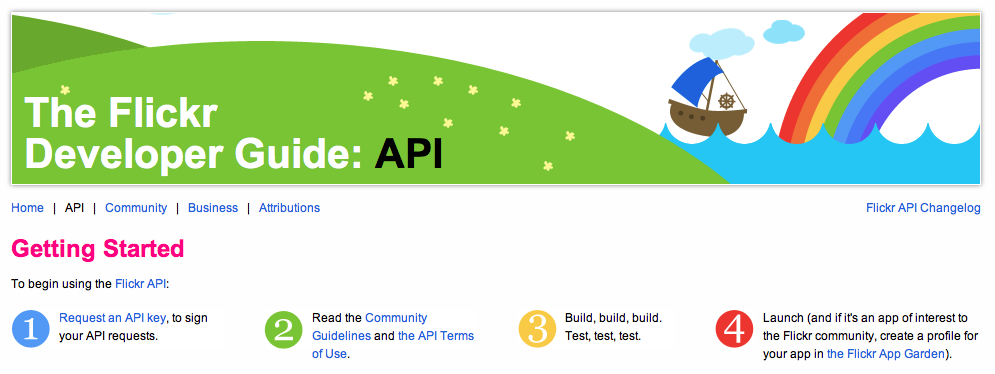
\includegraphics[width=\textwidth]{flickr_api.png}
  \end{center}

\end{frame}


\begin{frame}
  \frametitle{SELECT * FROM Internet\footnote{\url{http://oreillynet.com/pub/e/1369}}}

  \begin{center}

    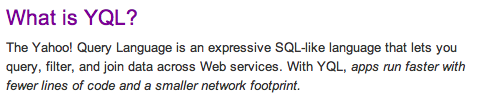
\includegraphics[width=\textwidth]{what_is_yql.png}
    \url{http://developer.yahoo.com/yql}

  \end{center}

\end{frame}


\begin{frame}
  \frametitle{YQL Console}

  \begin{center}
    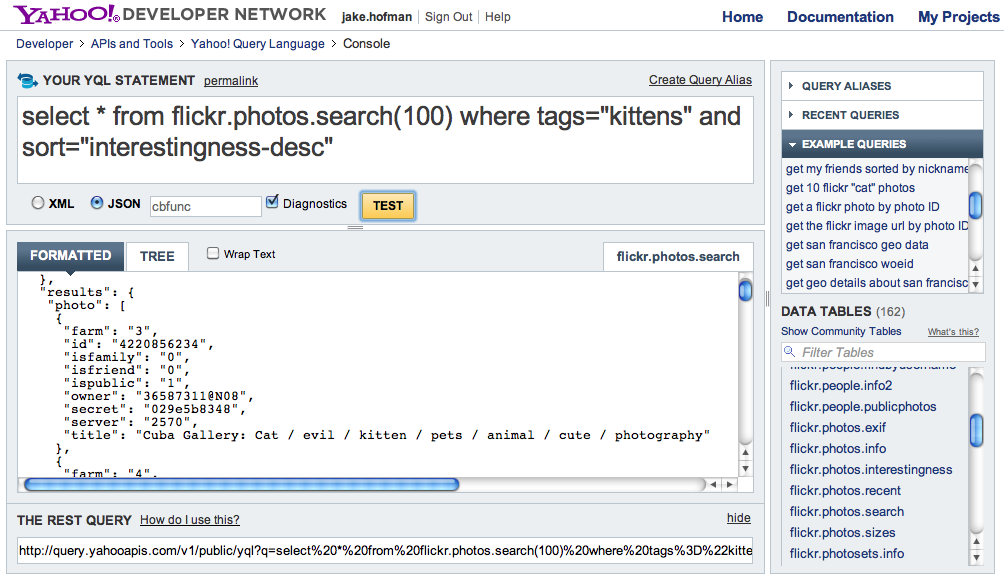
\includegraphics[width=\textwidth]{yql_console.png}
    \url{http://developer.yahoo.com/yql/console}
  \end{center}

\end{frame}


\begin{frame}[fragile]
  \frametitle{YQL + Python\footnote{See \url{http://python-yql.org/} for a more robust client}}

    \begin{block}{Python function for public YQL queries}
        \begin{lstlisting}[language=python]
YQL_PUBLIC = 'http://query.yahooapis.com/v1/public/yql'

def yql_public(query):
  # escape query
  query_str = urlencode({'q': query, 'format': 'json'})

  # fetch results
  url = '%s?%s' % (YQL_PUBLIC, query_str)
  result = urlopen(url)

  # parse json and return
  return json.load(result)['query']['results']

        \end{lstlisting}
    \end{block}
\end{frame}

\begin{frame}[fragile]
  \frametitle{YQL + Python + Flickr}

    \begin{block}{Fetch info for ``interestingness'' photos}
      \begin{lstlisting}[language=bash]
 ./simpleyql.py ``select * from
   flickr.photos.interestingness(100)''
      \end{lstlisting}
    \end{block}

    \begin{block}{Download thumbnails for photos tagged with ``vivid''}
      \begin{lstlisting}[language=bash]
 ./download_flickr.py vivid 500
      \end{lstlisting}
    \end{block}

\end{frame}


% todo: command line hack to get images from page?

\section{Image features}
\begin{frame}
  \frametitle{Images as arrays}

  \begin{center}
    Grayscale images $\leftrightarrow$ 2-d arrays of $M \times N$ pixel intensities
    \vskip20pt
    \only<1>{
\includegraphics[height=0.5\textheight]{../../code/image_data/sample_digit.png}}
    \only<2>{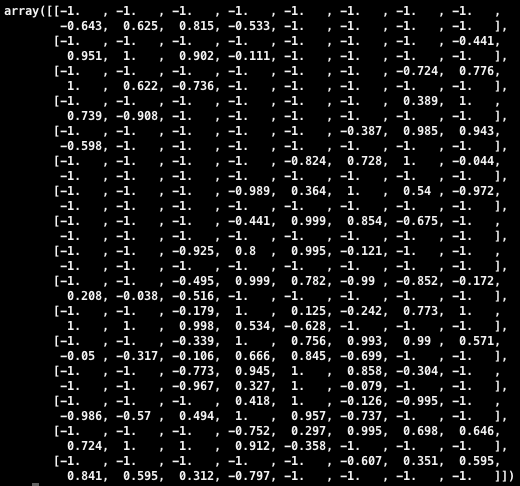
\includegraphics[height=0.5\textheight]{image_array.png}}
  \end{center}

\end{frame}

\begin{frame}[fragile]
  \frametitle{Images as arrays}

  \begin{center}
    Color images $\leftrightarrow$ 3-d arrays of $M \times N \times 3$ RGB pixel intensities
    \vskip20pt
    \only<1>{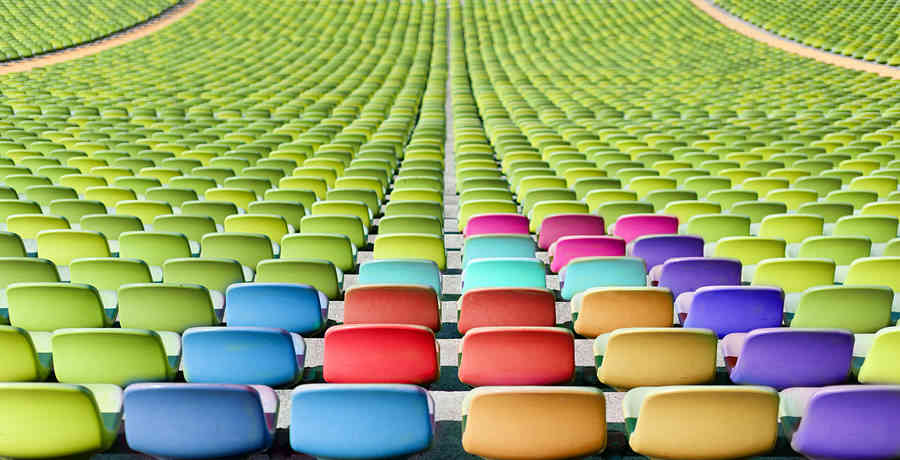
\includegraphics[height=0.45\textwidth]{../../code/image_data/chairs.jpg}}
    \only<2>{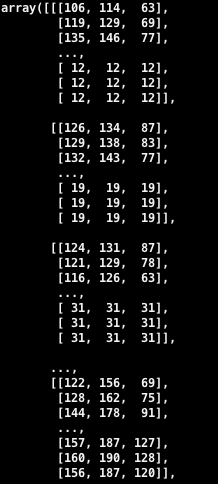
\includegraphics[height=0.5\textheight]{image_array_color.png}}
  \end{center}

    \begin{block}{}
        \begin{lstlisting}[language=python]
import matplotlib.image as mpimg
I = mpimg.imread('chairs.jpg')
        \end{lstlisting}
    \end{block}

\end{frame}


\begin{frame}
  \frametitle{Intensity histograms}

  \begin{center}
    Disregard all spatial information, simply count pixels by intensities \\
    (e.g. lots of bright green and dark blue pixels)
    \vskip20pt
  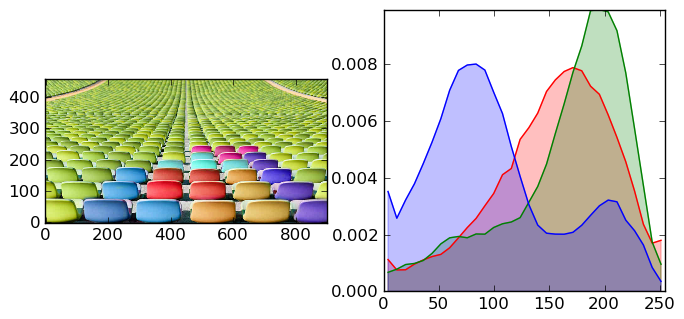
\includegraphics[width=\textwidth]{../../code/image_data/chairs_32.png}
  \end{center}

\end{frame}


\begin{frame}
  \frametitle{Intensity histograms}

  \begin{center}
    How many bins for pixel intensities?
    \vskip20pt
    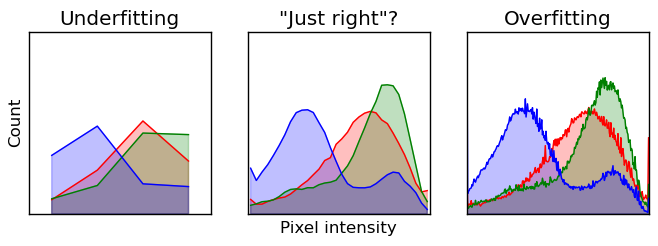
\includegraphics[width=0.75\textwidth]{chairs_hists.png}
    \vskip20pt
    \textbf{Too many} bins gives a noisy, \textbf{overly complex} representation of the data,\\
    while using \textbf{too few} bins results in an \textbf{overly simple} one
  \end{center}

\end{frame}



\section{Clustering}
\begin{frame}
  \frametitle{Clustering images}

  \begin{center}
    Clustering is an \textit{unsupervised} learning task by which we
    look for structure in the data, grouping similar examples together
    \vskip20pt
    \only<1>{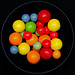
\includegraphics[height=0.25\textheight]{../../code/image_data/candy.jpg}}
    \only<2>{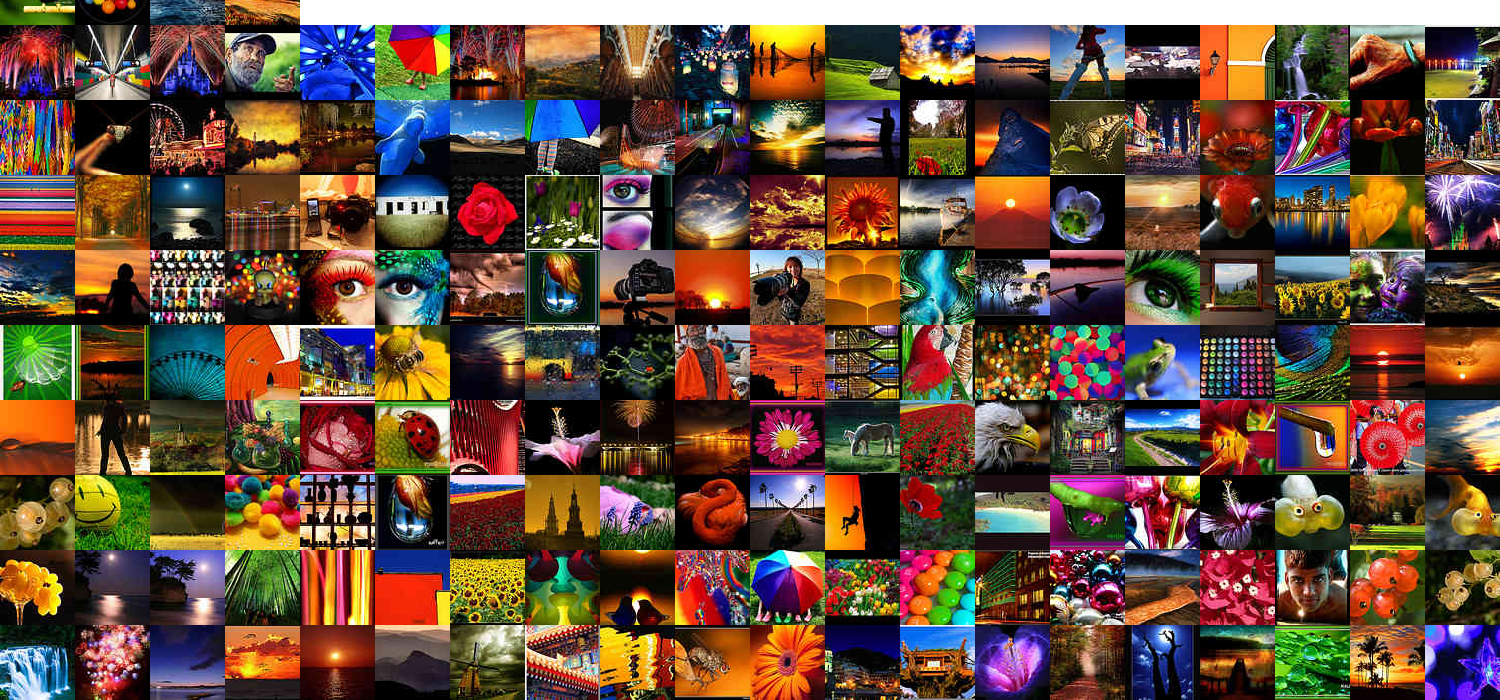
\includegraphics[height=0.25\textheight]{../../code/image_data/flickr_vivid_cluster_0}}
    \vskip20pt
    \only<1>{e.g., find groups of similar pixels within a single image}
    \only<2>{e.g., find groups of similar images across a collection of images}
  \end{center}

\end{frame}


\begin{frame}
  \frametitle{K-means clustering}

  \begin{center}
    K-means: represent each cluster by the average of its points 
    \vskip20pt
    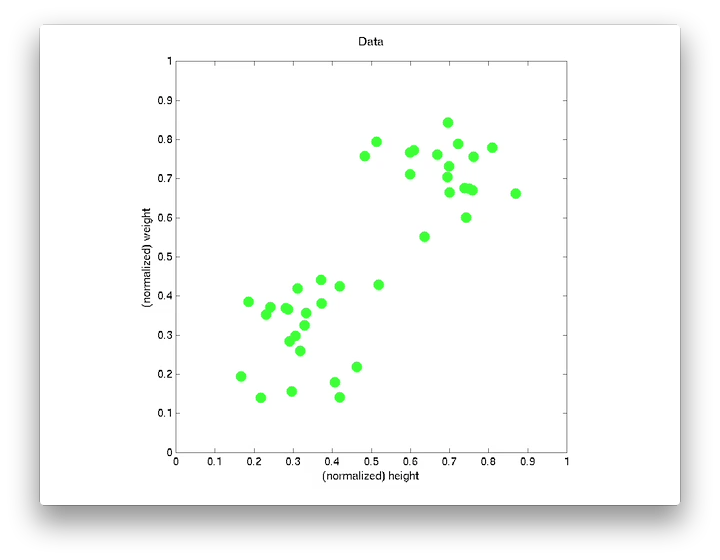
\includegraphics[width=0.6\textwidth]{em_animation_1.png}
    \vskip20pt
    Learn by iteratively updating cluster means and point assigments
  \end{center}
  % jntj: min inter-cluster var
\end{frame}

\begin{frame}[fragile]
  \frametitle{K-means clustering}

  \begin{center}

    \begin{columns}[c]
      
      \column{0.5\textwidth}
        K-means: \\
        \alert<1>{Choose number of clusters} \\
        \alert<1>{Initialize cluster centers} \\
        While not converged: \\
          \alert<2,4>{\hskip10pt Assign each point to closest cluster} \\
          \alert<3,5>{\hskip10pt Update cluster centers}

      \column{0.6\textwidth}

    \only<1>{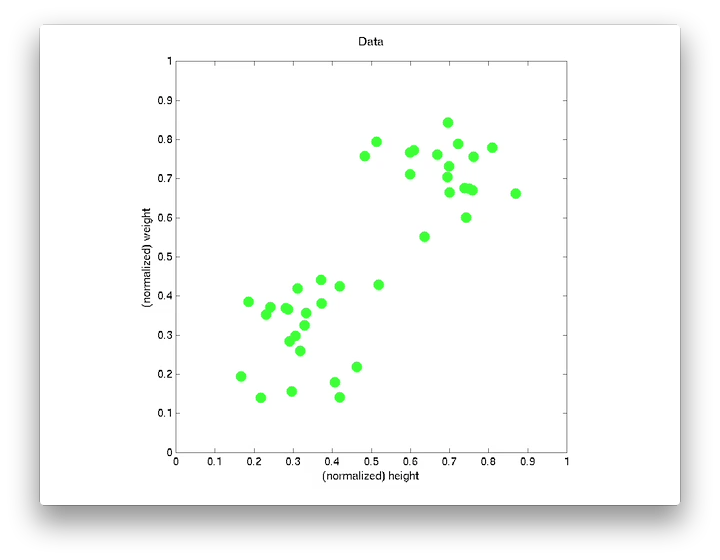
\includegraphics[width=1\textwidth]{em_animation_1.png}}
    \only<2>{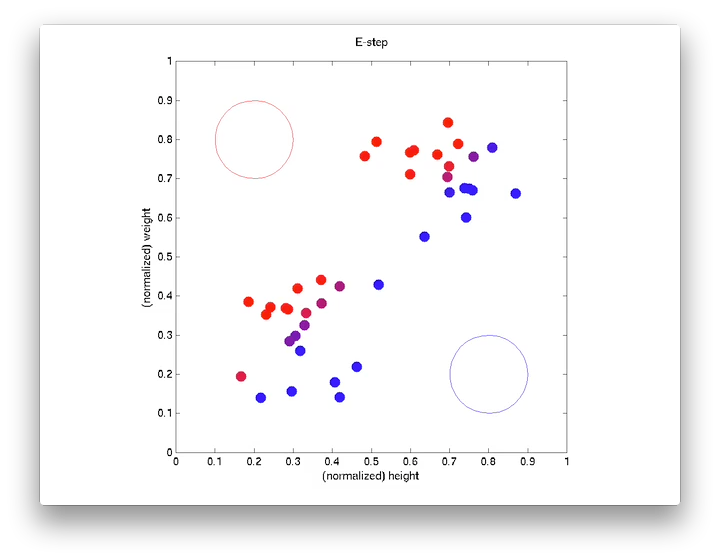
\includegraphics[width=1\textwidth]{em_animation_2.png}}
    \only<3>{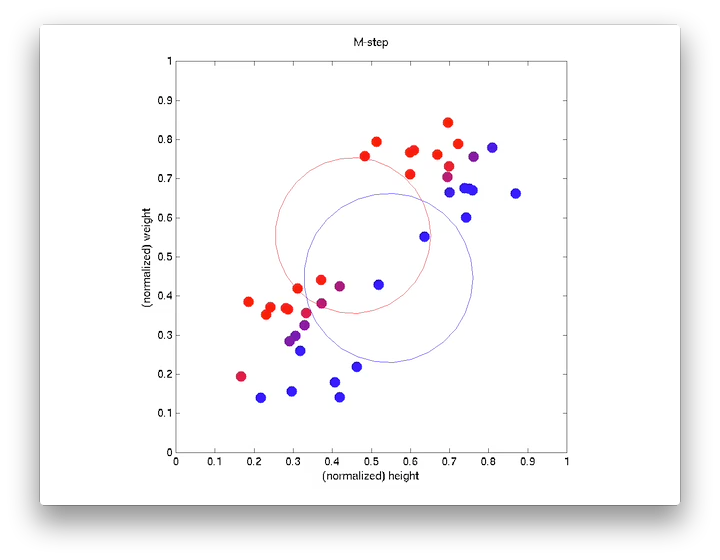
\includegraphics[width=1\textwidth]{em_animation_3.png}}
    \only<4>{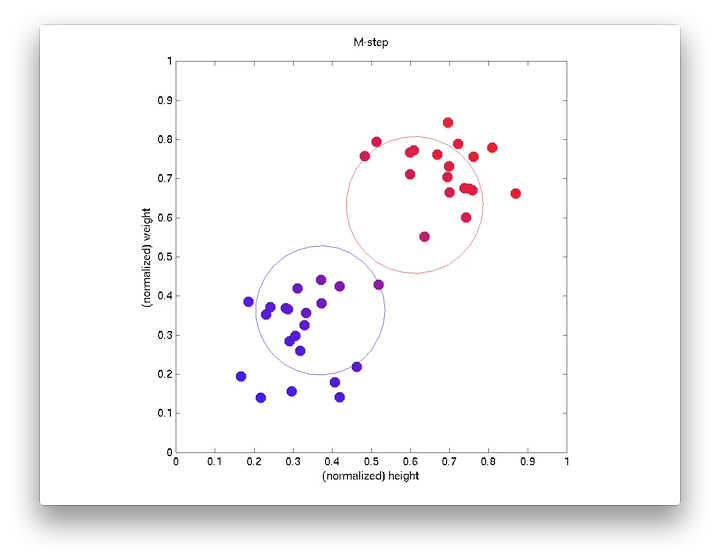
\includegraphics[width=1\textwidth]{em_animation_4.png}}
    \only<5>{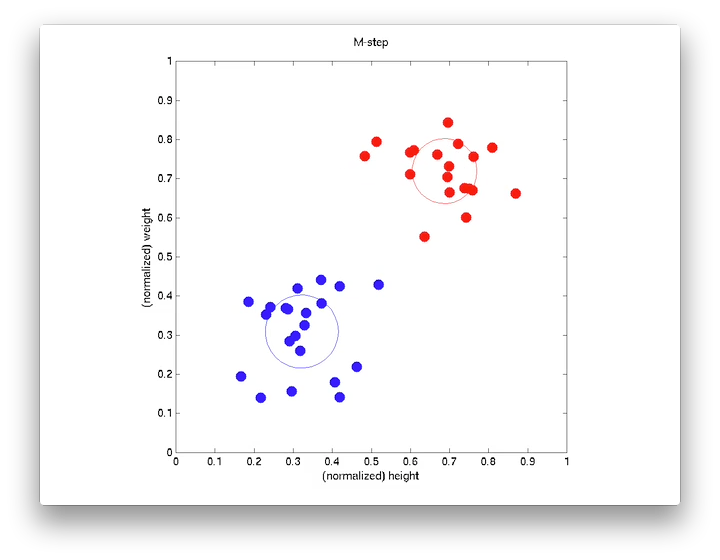
\includegraphics[width=1\textwidth]{em_animation_5.png}}

    \end{columns}
  \end{center}


\end{frame}


\begin{frame}
  \frametitle{Clustering pixels}

  \begin{center}
    Find groups of similar pixels within a single image \\
    (e.g. ``the bright red circles'')
    \vskip20pt
    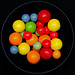
\includegraphics[height=0.25\textheight]{../../code/image_data/candy.jpg}
    \vskip20pt
    Represent each pixel as a separate example \\
    with its (R,G,B) value as a 3-d feature vector
  \end{center}

\end{frame}


\begin{frame}[fragile]
  \frametitle{Clustering pixels}

  \begin{center}

    \begin{block}{Group pixels within candy.jpg into 7 clusters}
        \begin{lstlisting}[language=bash]
 ./cluster_pixels.py candy.jpg 7
        \end{lstlisting}
    \end{block}
    \vskip20pt
    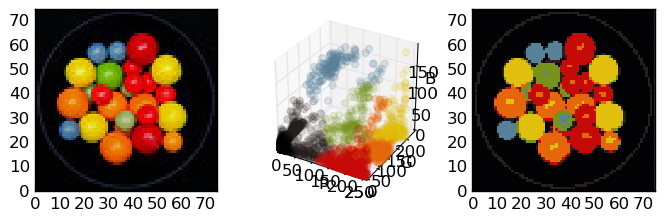
\includegraphics[width=\textwidth]{../../code/image_data/candy_clustered.png}
  \end{center}

\end{frame}

\begin{frame}
  \frametitle{Clustering images}

  \begin{center}
    Find groups of similar images within a collection of images \\
    (e.g. ``warm sunsets'')
    \vskip20pt
    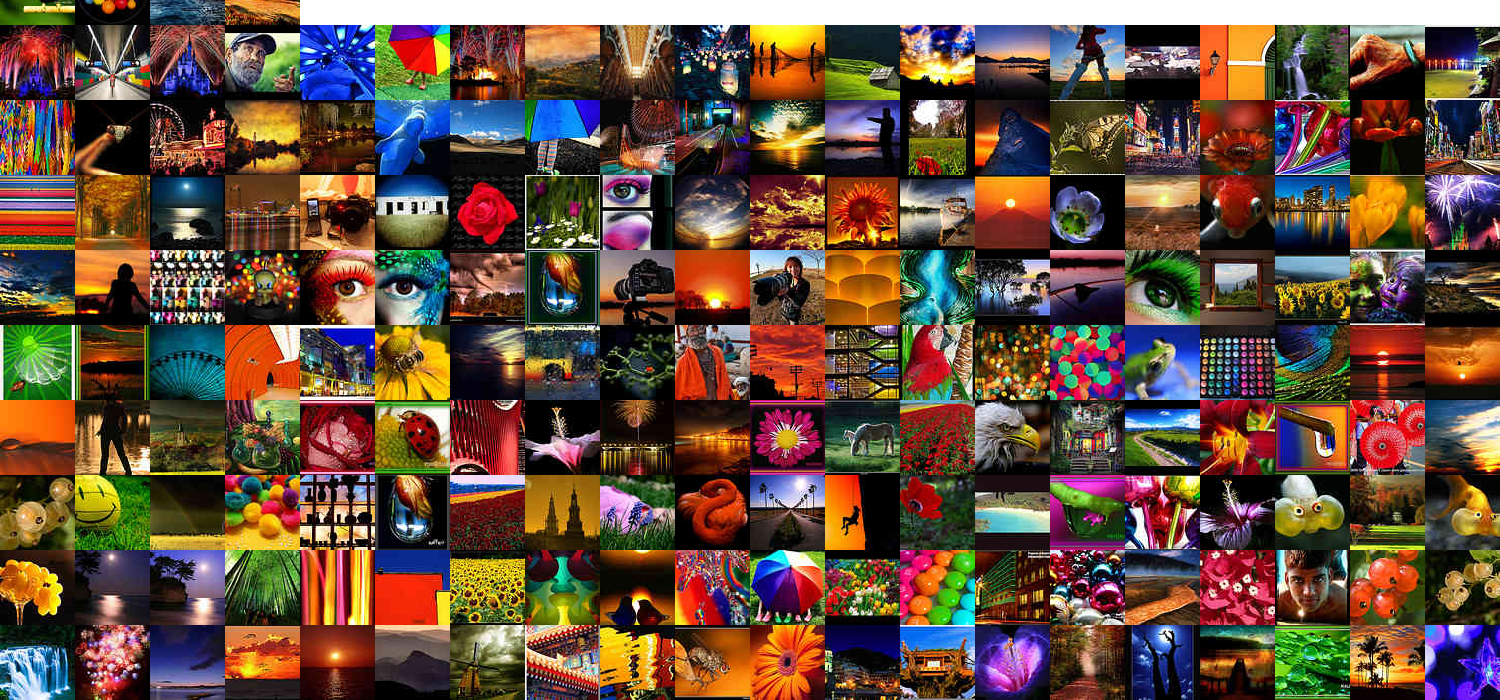
\includegraphics[height=0.25\textheight]{../../code/image_data/flickr_vivid_cluster_0.png}
    %\includegraphics[width=\textwidth]{flickr_vivid_clusters.pdf}
    \vskip20pt
    Represent each image with a binned RGB intensity histogram
  \end{center}

\end{frame}


\begin{frame}[fragile]
  \frametitle{Clustering images}

  \begin{center}

    \begin{block}{Group 'vivid' images into 3 clusters}
        \begin{lstlisting}[language=bash]
 ./cluster_flickr.py flickr_vivid 3 10
        \end{lstlisting}
    \end{block}
    \vskip20pt
    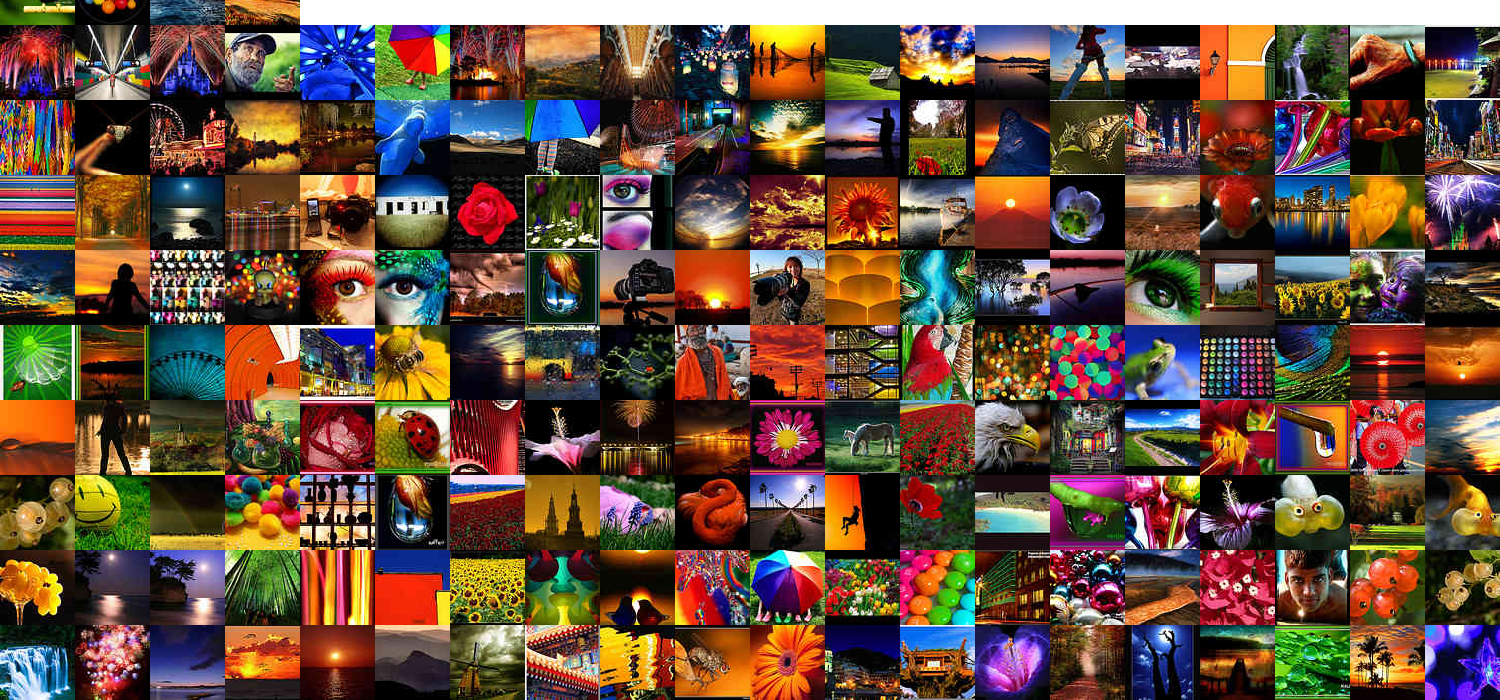
\includegraphics[height=0.2\textheight]{../../code/image_data/flickr_vivid_cluster_0.png}
    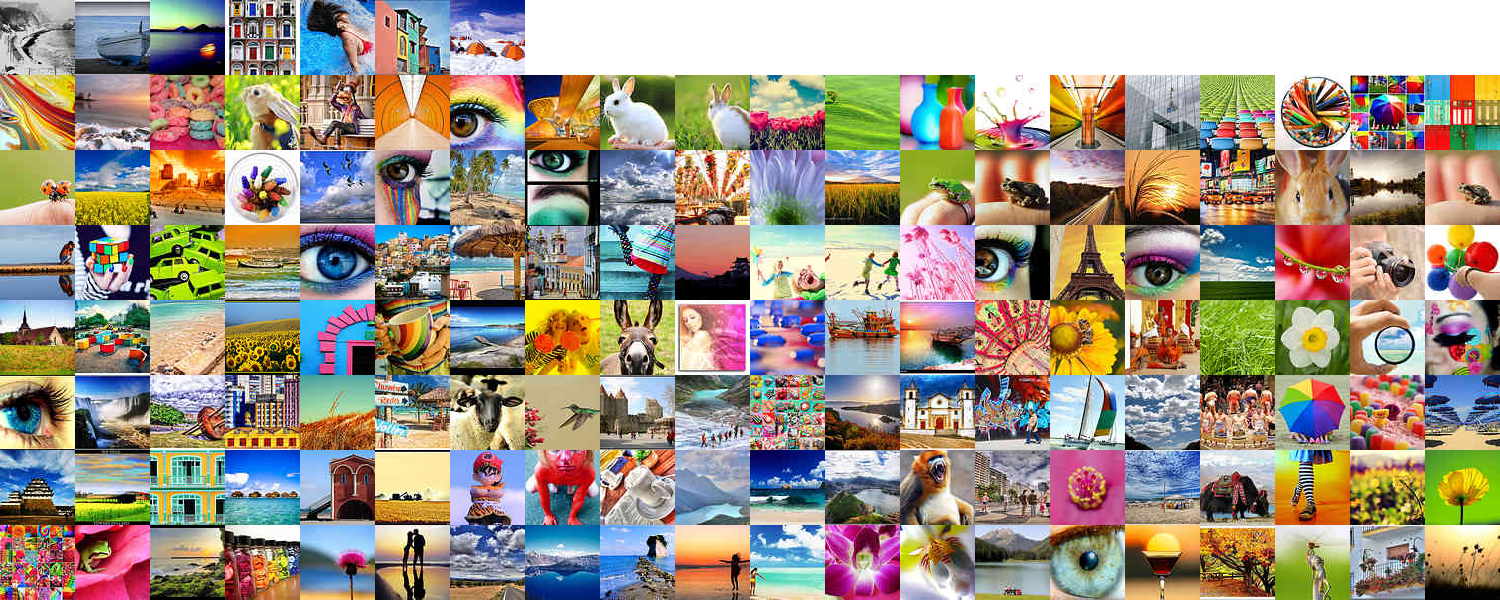
\includegraphics[height=0.2\textheight]{../../code/image_data/flickr_vivid_cluster_1.png}
    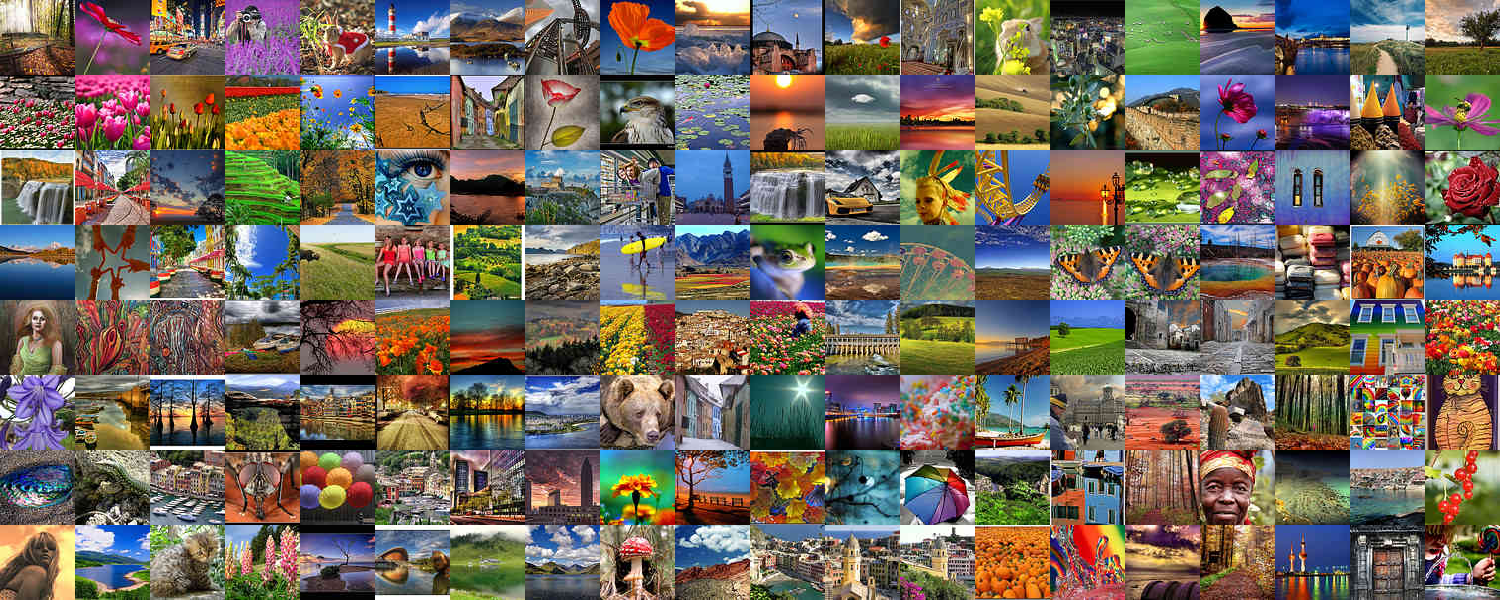
\includegraphics[height=0.2\textheight]{../../code/image_data/flickr_vivid_cluster_2.png}

  \end{center}

\end{frame}


\section{Classification}
\begin{frame}
  \frametitle{Classifying images}

  \begin{center}
    Classification is an \textit{supervised} learning task by which we
    aim to predict the correct label for an example given its features
    \vskip20pt

    \only<1>{
    
\includegraphics[width=0.5\textwidth]{ocr.png} \\
    \Huge{$\downarrow$} \\
    \Huge{0 \hskip10pt 5 \hskip10pt 4 \hskip10pt 1 \hskip10pt 4 \hskip10pt 9}
    \vskip20pt
    \normalsize
    e.g. determine which digit $\{0,1,\ldots,9\}$ is in depicted in each image
    }

    \only<2>{
      \begin{tabular}{cc}
        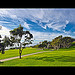
\includegraphics[height=0.2\textheight]{landscape.jpg} & 
\includegraphics[height=0.2\textheight]{headshot.jpg} \\
        $\downarrow$ & $\downarrow$ \\
        'landscape' & 'headshot'
      \end{tabular}
    \vskip20pt
    \normalsize
    e.g. determine if an image is a landscape or headshot
    }

  \end{center}

\end{frame}


\begin{frame}
  \frametitle{k-nearest neighbors classification}

  \begin{center}
    k-nearest neighbors: memorize training examples, predict labels using labels of the k closest training points
    \vskip20pt
    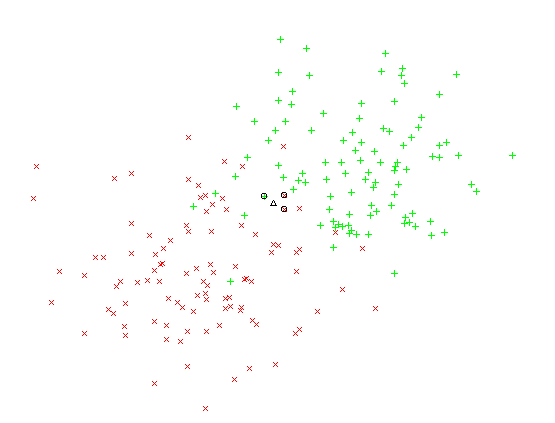
\includegraphics[width=0.65\textwidth]{knn_schematic.png}
    \vskip10pt
    Intuition: nearby points have similar labels
  \end{center}

\end{frame}


\begin{frame}
  \frametitle{k-nearest neighbors classification}

  \begin{center}
    %\vskip20pt
    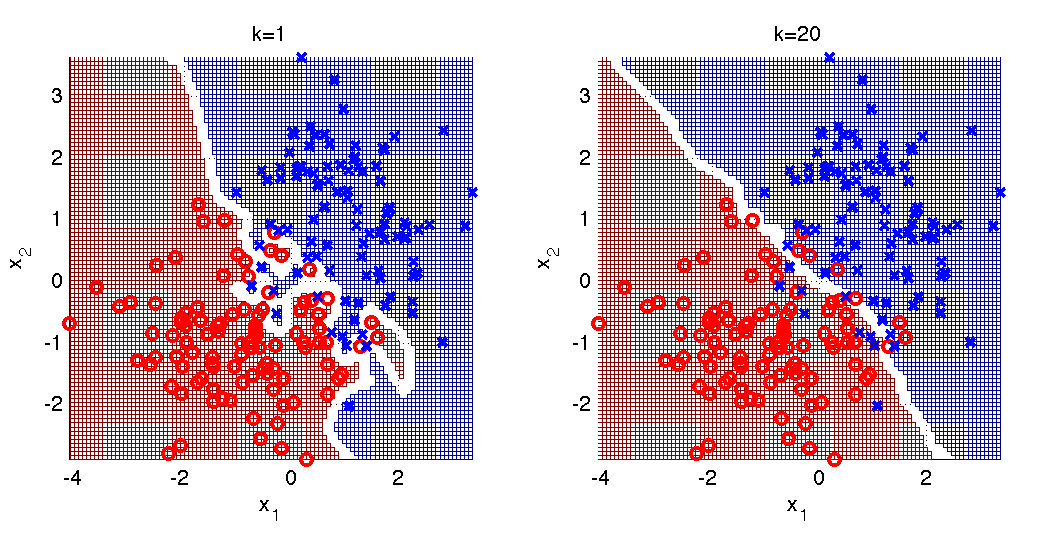
\includegraphics[width=\textwidth]{knn_boundary.png}
    \vskip10pt
    \textbf{Small k} gives a \textbf{complex} boundary, \textbf{large
      k} results in \textbf{coarse} averaging
  \end{center}

\end{frame}

\begin{frame}[fragile]
  \frametitle{k-nearest neighbors classification}

  \begin{center}
    \begin{block}{A simple kNN implementation with SciPy}
        \begin{lstlisting}[language=python]
import scipy.spatial as spat

# use the cdist function to quickly compute distances
# between all test and training examples
D = spat.distance.cdist(X, self.X, 'euclidean')

for i in range(N):
    # grab the indices of the k closest points
    ndx = D[i,:].argsort()[:k]

    # take a majority vote over the nearest points'
    # labels
    yhat[i] = mode(self.y[ndx])[0]
        \end{lstlisting}
    \end{block}
  \end{center}
\end{frame}


\begin{frame}
  \frametitle{Digit recognition}

  \begin{center}
    Determine which digit $\{0,1,\ldots,9\}$ is in depicted in each image
    \vskip10pt
    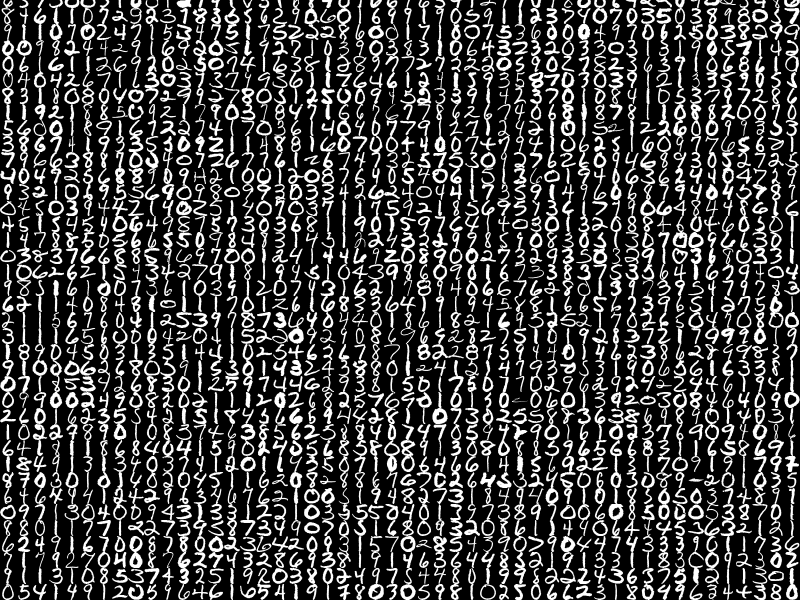
\includegraphics[width=0.65\textwidth]{../../code/image_data/sample_digits.png}
    %
\includegraphics[width=0.5\textwidth]{ocr.png} \\
    %\Huge{$\downarrow$} \\
    %\Huge{0 \hskip10pt 5 \hskip10pt 4 \hskip10pt 1 \hskip10pt 4 \hskip10pt 9}
    %\vskip20pt
    %\normalsize
    \vskip10pt
    Represent each image as a ``bag of pixels'', flattening the 2-d array
    of pixels to a 1-d vector

  \end{center}
\end{frame}


\begin{frame}[fragile]
  \frametitle{Digit recognition}

  \begin{center}
    \begin{block}{Simple digit classifer with k=1 nearest neighbors}
        \begin{lstlisting}[language=bash]
 ./classify_digits.py
        \end{lstlisting}
    \end{block}
    \vskip20pt
    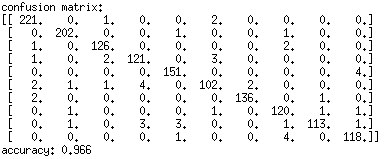
\includegraphics[width=0.55\textwidth]{digits_confmat.png}
  \end{center}
\end{frame}



\begin{frame}
  \frametitle{Image classification}

  \begin{center}
    Determine if an image is a landscape or headshot
    \vskip20pt
      \begin{tabular}{cc}
        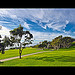
\includegraphics[height=0.2\textheight]{landscape.jpg} & 
\includegraphics[height=0.2\textheight]{headshot.jpg} \\
        $\downarrow$ & $\downarrow$ \\
        'landscape' & 'headshot'
      \end{tabular}
    \vskip20pt
    Represent each image with a binned RGB intensity histogram

  \end{center}
\end{frame}


\begin{frame}[fragile]
  \frametitle{Image classification}

  \begin{center}
    \begin{block}{Classify}
        \begin{lstlisting}[language=bash]
 ./classify_flickr.py 16 9 
    flickr_headshot flickr_landscape
        \end{lstlisting}
    \end{block}
    \vskip20pt
    \begin{block}{Change in performance with number of neighbors}
        \begin{lstlisting}[language=bash]
k = 1, accuracy = 0.7125
k = 3, accuracy = 0.7425
k = 5, accuracy = 0.7725
k = 7, accuracy = 0.7650
k = 9, accuracy = 0.7500
        \end{lstlisting}
    \end{block}
    %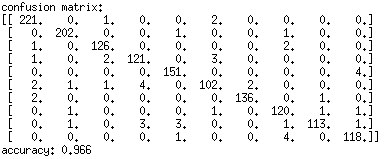
\includegraphics[width=0.55\textwidth]{digits_confmat.png}
  \end{center}
\end{frame}


\end{document}


